\subsection*{Квадратичные формы}
\begin{definition}
  Базис пространства $L$ называется \textit{согласованным} с подпространством $L_1$, если $L_1$ является линейной оболочкой какой"=то части базисных векторов.
\end{definition}
\begin{figure}[H]
  \centering
  \begin{subfigure}[b]{0.4\textwidth}
    \centering
    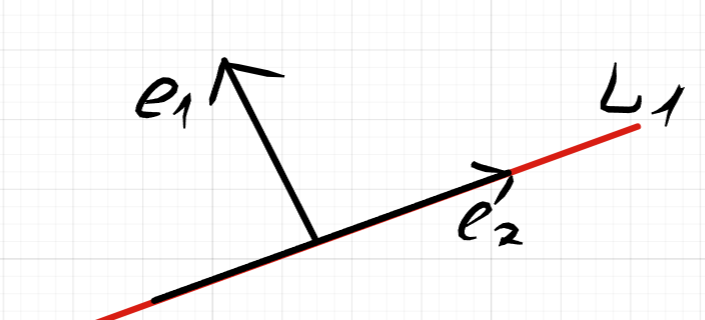
\includegraphics[width = \textwidth]{images/map_form_soglBasis.png}
    \caption{Пример согласованного базиса, так как $L_1 = <\!e_2\!>$}
  \end{subfigure}
  \hfill
  \begin{subfigure}[b]{0.4\textwidth}
    \centering
    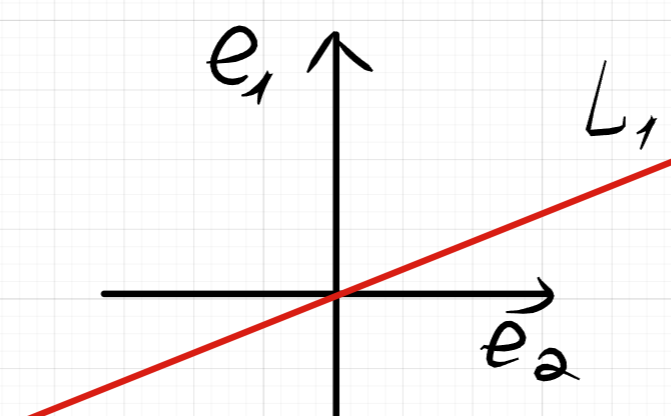
\includegraphics[width = \textwidth]{images/map_form_NesoglBasis.png}
    \caption{Пример несогласованного базиса}
  \end{subfigure}
\end{figure}

\begin{definition}
  \textit{Суммой} подпространств $L_1,L_2, \ldots, L_k$ называется совокупность векторов вида $\bar{u}_1 + \bar{u}_2 + \ldots + \bar{u}_k$, где $\bar{u}_i \in L_i,~ i = 1,\ldots,k.$
\end{definition}


\begin{theorem}
  Для всякой пары подпространств $L_1,\; L_2 \in L$ существует базис пространства $L$, согласованный с подпространствами $L_1,\;L_2$.
\end{theorem}
\begin{Proof}
  Пусть $(\bar{e}_1, \ldots, \bar{e}_k)$ "--- базис $L_1 \cap L_2$.Дополним до базиса $L_1$ и $L_2$:

  $(\bar{e}_1, \ldots, \bar{e}_k, \bar{f}_1, \ldots, \bar{f}_m)$ "--- базис $L_1$.

  $(\bar{e}_1,\ldots, \bar{e}_k, \bar{d}_1, \ldots, \bar{d}_p)$ "--- базис $L_2$.

  Рассмотрим $(\bar{e}_1, \ldots, \bar{e}_k, \bar{f}_1, \ldots, \bar{f}_m,\bar{d}_1, \ldots, \bar{d}_p)$ и докажем, что векторы линейно независимы.
  \begin{gather*}
    \sum_{j = 1}^{k}\lambda_j \, \bar{e}_j + \sum_{j = 1}^{m} \mu_j \, \bar{f}_j + \sum_{j = 1}^{p} \nu_j \, \bar{d}_j = 0 \\
    \underbrace{\sum_{j = 1}^{k}\lambda_j \, \bar{e}_j + \sum_{j = 1}^{m} \mu_j \, \bar{f}_j}_{\in \, L_1} = \underbrace{-\sum_{j = 1}^{p} \nu_j \, \bar{d}_j}_{\in \, L_2} 
  \end{gather*}
  Векторы $(d_1, \ldots, d_p) \notin L_1 \cap L_2 \implies$ равенство возможно только, если все коэффициенты равны нулю, то есть векторы линейно независимы.
\end{Proof}

\begin{corollary}
  $dim\,(L_1 + L_2) = dim\,L_1 + dim\,L_2 - dim\,(L_1 \cap L_2)$  
\end{corollary}

\begin{definition}
  Подпространства $L_1, \ldots, L_k$ называются \textit{линейно независимыми}, если из равенства $\bar{u}_1 + \bar{u}_2 + 
  \ldots + \bar{u}_k = \bar{0},~ \bar{u}_i \in L_i$ следует $\bar{u}_1 = \bar{u}_2 = \ldots = \bar{u}_k = \bar{0}$. 
\end{definition}

\begin{definition}
  Векторное пространство $L$ \textit{разлагается} в прямую сумму подпространств $L_1, \ldots, L_k$, если 
  \begin{enumerate}
    \item $L_1, \ldots, L_k$ "--- линейно независимые
    \item $L_1 + \ldots + L_k = L$
  \end{enumerate}
  Обозначение: $L = L_1 \oplus L_2 \oplus \ldots \oplus L_k$.
\end{definition}
$\forall \bar{v} \in L ~ \bar{v} = \bar{u}_1 + \bar{u}_2 + \ldots + \bar{u}_k,~ \bar{u}_i \in L_i ~ u_i$ называется \textit{проекцией} $v$ на $L_i$.

Напомним, что \textit{линейной} функией называют функцию $\alpha: V \to \Real$, где $V$ "--- векторное пространство (Далее $L,\; V, \; L_i, \; V_i$ "--- векторные пространства), если выполняются следующие условия:
\begin{enumerate}
  \item $\alpha(\bar{x} + \bar{y}) = \alpha(\bar{x}) = \alpha(\bar{y})$
  \item $\alpha(\lambda \bar{x}) = \lambda \alpha(\bar{x})$.
\end{enumerate}
$\forall \, \bar{x},\; \bar{y} \in V$.
\begin{example}
  \textit{След квадратной матрицы} "--- это сумма её диагональных элементов.
  $tr\, A = a_1^1 + a_2^2 + \ldots + a_n^n$

  След квадратной матрицы есть линейная функция, заданная на множестве квадратных матриц. $\alpha(A) = tr\,A , ~ V = M_{m \times n}$.
\end{example}

\begin{definition}
  Линейные функции \textit{образуют} подпространство в пространстве всех функций, заданных на $V$ со значениями $\Real$. 

  Пространство линейных функций, заданных на $V$, называется \textit{сопряженным пространством} по отношению $V$. Обозначение: $V^{\ast}$.
\end{definition}

Пусть $(\bar{e}_1, \ldots, \bar{e}_n)$ "--- базис $V$, а $(\eps_1, \ldots, \eps_n)$ "--- базис $V^{\ast}$.

$\eps_{i} \, (\bar{e}_j) = \delta_{ij} = \begin{cases}
  1&, \text{если } i = j \\
  0&, \text{если } i \neq j.
\end{cases} ~~\text{(символ Кронекера)}$

$\eps_i(\bar{x}) = x_i$.

Напомним также, что \textit{билинейной} функцией (формой) называется функция $\alpha: V \times V \to \Real$, которая линейна по каждому аргументу.

Примером билинейной функции является след: $\alpha(A,B) = tr \, (AB)$.

\begin{definition}
  \textit{Ядром} билинейной функии называется подпространство $Ker\, \alpha = \{\bar{y},~ \alpha(\bar{x}, \bar{y}) = 0,~ \forall \, \bar{x} \in V \}$.
\end{definition}
\begin{definition}
  Функция $\alpha$ называется \textit{невырожденной}, если ядро состоит из нуля ($Ker\, \alpha = 0$).
\end{definition}

Функция $\alpha$ является симметрической, если $\alpha(\bar{x}, \bar{y}) = \alpha(\bar{y}, \bar{x})$.

Функция $\alpha$ является кососимметрической, если $\alpha(\bar{x}, \bar{y}) = -\alpha(\bar{y}, \bar{x})$.

\begin{definition}
  Пусть $\alpha$ симметрическая билинейная функция над полем $K,~ char\, K \neq 2$. Функция $q: V \to K$, которая определяется как $q(\bar{x}) = \alpha(\bar{x}, \bar{x})$, называется \textit{квадратичной} функцией или формой, ассоциированной с функцией $\alpha$
\end{definition}

В координатной форме квадратичную функцию можно записать так:
$$
  q(\bar{x}) = \sum_{i,\, j} a_{ij}\,x_i\, x_j
$$

Симметрическая билинейная функция может восстанавливаться по соответствующей квадратичной функции.
$\alpha(\bar{x},\, \bar{y}) = \frac{1}{2} (q(\bar{x} + \bar{y}) - q(\bar{x}) - q(\bar{y}))$.
\begin{Proof}
  \begin{gather*}
    q(\bar{x} + \bar{y}) = \alpha(\bar{x} + \bar{y},\, \bar{x} + \bar{y}) = \\
    = \alpha(\bar{x}, \, \bar{x}) + \alpha(\bar{y},\, \bar{x}) + \alpha(\bar{x}, \, \bar{y}) + \alpha(\bar{y}, \, \bar{y}) = \\
    = \alpha(\bar{x}, \, \bar{x}) + \alpha(\bar{y}, \, \bar{y}) + 2\alpha(\bar{x}, \, \bar{y}) \implies \\
    2\alpha(\bar{x}, \, \bar{y}) = q(\bar{x} + \bar{y}) - q(\bar{x}) - q(\bar{y})
  \end{gather*}
\end{Proof}

\begin{definition}
  Векторы $\bar{x}$ и $\bar{y}$ называются \textit{ортогональными}, если $\alpha(\bar{x}, \, \bar{y}) = 0$.
\end{definition}

\begin{definition}
  \textit{Ортогональным дополнением} к подпространству $U$ относительно $\alpha$ называется подпространство $U^+ = \{\bar{y}:~ \alpha(\bar{x}, \, \bar{y}) = 0, ~ \forall \, \bar{x} \in U\}$.

  Заметим, что $U^{+} = Ker\; \alpha$.
\end{definition}  

\begin{figure}[H]
  \centering
  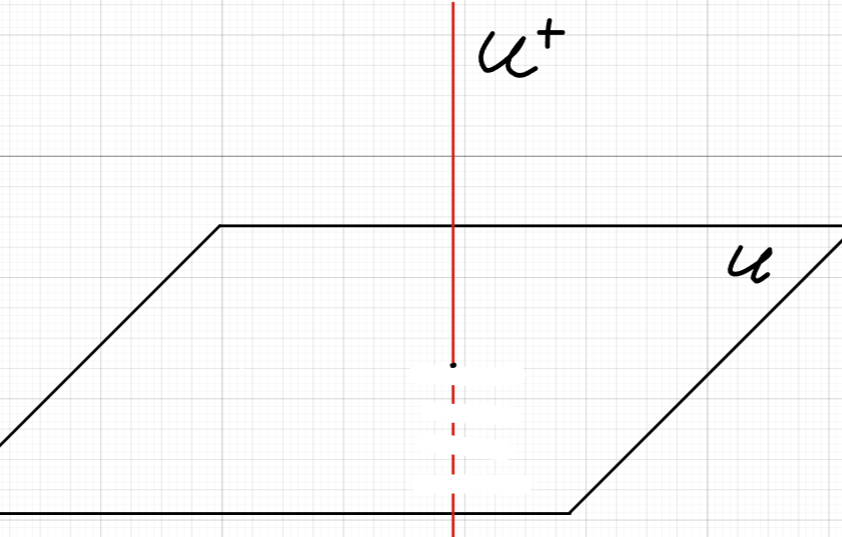
\includegraphics[height = 3cm]{images/map_form_ortog.png}
  \caption{Пример ортогонального дополнения к $U$ относительно скалярного произведения}
\end{figure}

\begin{definition}
  Подпространство $U$ называется \textit{невырожденным} относительно билинейной функции $\alpha$, елси её ограничения на $U$ невырожденно
\end{definition}

\begin{definition}
  Пусть $\alpha$ "--- симметрическая билинейная форма. Базис $(\bar{e}_1, \ldots, \bar{e}_n)$ называется \textit{ортогональным} относительно $\alpha$, если его векторы попарно ортогональны.

\end{definition}
В ортогональном базисе верны следующие утверждения:
\begin{itemize}
  \item[] $\alpha(\bar{x}, \, \bar{y}) = \alpha_1 \, x_1 \, y_1 + \ldots + \alpha_n \, x_n \, y_n$
  \item[] $q(\bar{x}) = \alpha(\bar{x}, \bar{x}) = \alpha_1 \, x_1^2 + \ldots + \alpha_n \, x_n^2$
  \item[] $\alpha(\bar{e}_i, \, \bar{e}_j) = 0$, если $i \neq j$
  \item[] $\alpha_i = \alpha(\bar{e}_i, \, \bar{e}_i)$
\end{itemize}

\begin{theorem}
  \label{theorem: gram_schmidt}
  Пусть $(\bar{e}_1, \bar{e}_2, \ldots, \bar{e}_n)$ "--- базис $V$, $A$ "--- матрица функции $\alpha$ в этом базисе, $A_k$ "--- матрица функции $\alpha$ на подпространстве $V_k = <\!\bar{e}_1, \ldots, \bar{e}_k \!>, ~ k \leq n$ и $\delta_k = det\,A_k$.

  Если все угловые миноры ($\delta_1, \ldots, \delta_n)$ отличны от нуля, то \textbf{сущестует} единственный ортогональный базис $(\bar{f}_1, \ldots, \bar{f}_n)$ удовлетворяющий условию $\bar{f}_k \in \bar{e}_k + V_{k - 1},~ k = 1, \ldots, n$.

  При этом $q(\bar{f}_k) = \alpha(\bar{f}_k, \, \bar{f}_k) = \frac{\delta_k}{\delta_{k - 1}}$.
\end{theorem}

\begin{definition}
  Процесс построения ортогонального базиса называется процессом \textit{ортогонализации Грама"=Шмидта}.
\end{definition}
\begin{example}
  Процесс ортогонализации Грама"=Шмидта:
  \begin{figure}[H]
    \centering
    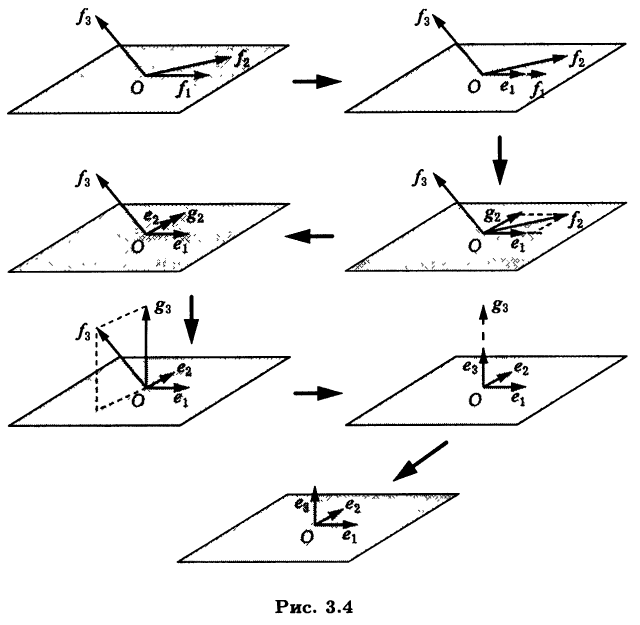
\includegraphics[width= \textwidth]{images/map_form_gram-shmidt.png}
  \end{figure}
\end{example}
Построение ортонормированного базиса:

$(\bar{e}_1, \ldots, \bar{e}_n)$ "--- базис $\rightarrow ~ (\bar{f}_1, \ldots, \bar{f}_n)$ "--- ортогональный базис ($\bar{f}_i \; \bot \; \bar{f}_j, ~ \alpha(\bar{f}_i, \, \bar{f}_j) = 0$ при $i \neq j$) $\rightarrow ~ (\bar{d}_1, \ldots, \bar{d}_n)$ "--- ортонормированный базис ($\mathopen| \bar{d}_i \mathclose| = 1$).

\begin{definition}
  Вещественная квадратичная форма $q$ называется \textit{положительно определенной}, если $q(\bar{x}) > 0,~ \bar{x} \neq \bar{0}$

  Вещественная симметрическая билинейная форма назыается \textit{положительно определенной}, если соответствующая ей квадратичная форма положительно определена.
\end{definition}
\begin{theorem}[Критерий Сильвестра]
  Вещественная квадратичная функция является \textbf{положительно определённой} тогда и только тогда, когда все угловые миноры её матрицы \textbf{положительны}.
\end{theorem}
\subsection*{Канонический вид квадратичных форм}

Если квадратичная функция $q: V \to \Complex$ определена на поле комплексных чисел, то путём нормировки базисных векторов квадратичную форму можно привести к виду 
$$q(\bar{x}) = x_1^2 + \ldots + x_r^2,$$ где $r$ "--- ранг квадратичной формы.

В случае же, когда квадратичная форма $q: V \to \Real$ определена на поле вещественных чисел, то форму можно привести к виду 
\begin{equation}
  \label{eq:quad_real}
  q(\bar{x}) = x_1^2 + x_2^2 + \ldots + x_k^2 - x_{k + 1}^2 - x_{k + 2}^2 - \ldots - x_{k + \ell}^2,
\end{equation}
где $k + \ell$ "--- ранг формы.

Число $k$ в нормальном виде квадратичной формы \ref{eq:quad_real} есть \textit{максимальная размерность подпространства}, на котором функция $q$ положительно определена.

\begin{theorem}[Закон инерции]
  Числа $k$ и $\ell$ в нормальном виде \ref{eq:quad_real} вещественной квадратичной функции не зависят от выбора базиса, в котором эта функция имеет нормальный вид.

  Пара $(k, \, \ell)$ называется \textbf{сигнатурой} квадратичной функции.
\end{theorem}

\subsection*{Евклидово пространство}

\begin{definition}
  \textit{Евклидовым векторным пространством} называется действительное векторное пространство с фиксированным положительно определенной симметрической билинейной функцией. Эта функция называется \textit{скалярным произведением}.
\end{definition}

\begin{definition}
  \textit{Матрицей Грама} (в евклидовом пространстве) называется $$
  G(\bar{e}_1, \ldots, \bar{e}_n) = \begin{pmatrix}
    (\bar{e}_1,\, \bar{e}_1) & (\bar{e}_1,\, \bar{e}_2) & \ldots & (\bar{e}_1,\, \bar{e}_n) \\
    (\bar{e}_2,\, \bar{e}_1) & (\bar{e}_2,\, \bar{e}_2) & \ldots & (\bar{e}_2,\, \bar{e}_n) \\
    \vdots & \vdots && \vdots \\
    (\bar{e}_n,\, \bar{e}_1) & (\bar{e}_n,\, \bar{e}_2) & \ldots & (\bar{e}_n,\, \bar{e}_n)
  \end{pmatrix},
  $$
  где $(\bar{e}_i,\, \bar{e}_j)$ "--- скалярное произведение. Так как функция симметрическая, то матрица симметрична относительно главной диагонали.
\end{definition}
(Не было на лекциях) Матрица Грама обладают следующими свойствами:
\begin{itemize}
  \item[] Определитель матрицы Грама системы $n$ векторов равен квадрату объёма 
  $n$"=мерного параллелепипеда, натянутого на эти векторы. Из этого следует, что в случае трёхмерного пространства определитель Грама трёх векторов равен квадрату их смешанного произведения.
  \item[] Система векторов $v_1, \ldots, v_n$ линейно зависима тогда и только тогда, когда определитель матрицы Грама этой системы равен нулю.
\end{itemize}

Пусть $L = U \oplus U^+ \implies \underbrace{\bar{x}}_{\in \, L} = \underbrace{\bar{y}}_{\in \, U} + \underbrace{\bar{z}}_{\in\, U_+}$, где $\bar{y}$ "--- ортогональная \textit{проекция} $\bar{x}$ на $U$, $\bar{z}$ "--- ортогональная \textit{составляющая} $\bar{x}$ относительно $U$.

Пусть $(\bar{e}_1, \ldots, \bar{e}_k)$ "--- ортогональный базис $U$.

Зная $\bar{x}$,
\textbf{Как найти проекцию и составляющую?}
\begin{gather*}
  \bar{x} = \lambda_1 \, \bar{e}_1 + \lambda_2 \, \bar{e}_2 + \ldots + \lambda_k \, \bar{e}_k + \bar{z} ~~/ \text{ Скалярно умножаем на } \bar{e}_1 \\
  (\bar{x}, \, \bar{e}_1) = \lambda_1(\bar{e}_1,\, \bar{e}_1) + \lambda_2\underbrace{(\bar{e}_1, \, \bar{e}_2)}_{ = \, 0} + \ldots + \lambda_k \underbrace{(\bar{e}_k, \, \bar{e}_1)}_{ = \, 0} + \underbrace{(\bar{z}, \, \bar{e}_1)}_{= \, 0} \\
  \lambda_1 = \frac{(\bar{x}, \, \bar{e}_1)}{\bar{e}_1^2} \\
  \text{Проделывая аналогочные действия для всех } i = 1, \ldots, k  \text{, получим:}\\
  \lambda_i = \frac{(\bar{x}, \bar{e}_i)}{\bar{e}_i^2} \\
  \implies \bar{x} = \underbrace{\sum_{i = 1}^{k} \frac{(\bar{x}, \, \bar{e}_i)}{(\bar{e}_i, \, \bar{e}_i)} \cdot \bar{e}_i}_{y} + \bar{z} \implies \bar{z} = \bar{x} - \bar{y}.  
\end{gather*}

По теореме \ref{theorem: gram_schmidt} мы знаем, когда существует ортогональный базис, но
\textbf{Как построить ортогональный базис?}

Пусть $(\bar{e}_1, \ldots, \bar{e}_n)$ "--- произвольный базис. Построим ортогональный базис $(\bar{f}_1, \ldots, \bar{f}_n)$.

$\bar{f}_1 = \bar{e}_1$

$\bar{e}_2 = \lambda_1 \, \bar{e}_1 + \bar{f}_2,$ где $\bar{f}_2$ "--- ортогональная составляющая. Умножаем выражение скалярно на $\bar{f}_1 = \bar{e}_1$ 

$(\bar{e}_2, \, \bar{f}_1) = \lambda_1 \, (\bar{e}_1, \, \bar{f}_1) + \underbrace{(\bar{f}_2,\, \bar{f}_1)}_{\substack{= \, 0, \\ \text{так как } \bar{f}_2 \; \bot \; \bar{f}_1}}$

$\lambda_1 = \frac{(\bar{e}_2, \, \bar{f}_1)}{(\bar{f}_1, \bar{f}_1)} \implies \bar{f}_2 = \bar{e}_2 - \lambda_1 \, \bar{e}_1$

$\bar{e}_3 = \lambda \, \bar{f}_1 + \mu \, \bar{f}_2 + \bar{f}_3$

Скалярно умножаем на $f_1$: $\lambda = \frac{(\bar{e}_3, \, \bar{f}_1)}{(\bar{f}_1, \, \bar{f}_1)}$

Скалярно умножаем на $f_2$: $\mu = \frac{(\bar{e}_3, \, \bar{f}_2)}{(\bar{f}_2, \, \bar{f}_2)}$

$\implies \bar{f}_3 = \bar{e}_3 - \lambda \, \bar{f}_1 - \mu \, \bar{f}_2$

Следовательно $\bar{f}_i = \bar{e}_i - \sum\limits_{k = 1}^{i - 1} \frac{(\bar{e}_i, \, \bar{f}_k)}{(\bar{f}_k, \, \bar{f}_ k)} \cdot \bar{f}_k, ~ i = 1, \ldots, n$

\begin{definition}
  Евклидовые векторные пространства $V, \, U$ называются изоморфными, если существует биективное отображение $f: V \to U$ являющаяся изоморфизмом и выполняется равенство $(f(\bar{a}), \, f(\bar{b})) = (\bar{a}, \bar{b}),~ \forall \, \bar{a}, \, \bar{b} \in V.$
\end{definition}

\begin{theorem}
  Любые два евклидовых векторных пространства одинаковой размерности изоморфны.
\end{theorem}
\begin{Proof}
  Пусть $dim \, V = dim \, U = n,~ U,\, V$ "--- векторные пространства,

  $(\bar{v}_1, \ldots, \bar{v}_n), \, (\bar{u}_1, \ldots, \bar{u}_n)$ "--- ортонормированные базисы $V$ и $U$ соответственно.

  Построим отображение
  $f: V \to U, ~f(\bar{v}_i) = \bar{u}_i,~$ а значит $(f(\bar{v}_i), \, f(\bar{v}_k)) = (\bar{u}_i, \, \bar{u}_k) = \delta_{ik} = (\bar{v}_i, \, \bar{v}_k)$.

  Следовательно $V$ и $U$ изоморфны.
\end{Proof}

\subsection*{Линейный оператор}
\begin{definition}
  \textit{Линейным оператором} или \textit{линейным преобразованием} векторного пространства $L$ называется линейное отображение в себя $A: L \to L$.
  
  Выполняются следующие условия:
  \begin{enumerate}
    \item $A(\bar{x} + \bar{y}) = A\, \bar{x} + A \, \bar{y}$
    \item $A(\lambda\bar{x}) = \lambda A\, \bar{x}$
  \end{enumerate}
\end{definition}

Пусть $(\bar{e}_1, \ldots, \bar{e}_n)$ "--- базис $L$,
\begin{gather*}
  A(\bar{e}_1) = a_1^1\bar{e}_1 + a_1^2\bar{e}_2 + \ldots + a_1^n\bar{e}_n \\
  \vdots \\
  A(\bar{e}_n) = a_n^1\bar{e}_1 + a_n^2\bar{e}_2 + \ldots + a_n^n \bar{e}_n \\
  \underbrace{(A\, \bar{e}_1, \ldots, A\, \bar{e}_n)}_{\text{матрица"=строка}} = \underbrace{(\bar{e}_1, \ldots, \bar{e}_n)}_{\text{матрица"=строка}} \cdot \begin{pmatrix}
    a_1^1 & \cdots & a_n^1 \\
    \vdots & \ddots & \vdots \\
    a_1^n & \cdots & a_n^n
  \end{pmatrix} \\
  A\, \bar{e}_i = \sum_{k = 1}^n \, a_i^k \bar{e}_k, ~ k = 1, \ldots, n 
\end{gather*}
\begin{definition}
  Матрица $\begin{pmatrix}
    a_1^1 & \cdots & a_n^1 \\
    \vdots & \ddots & \vdots \\
    a_1^n & \cdots & a_n^n
  \end{pmatrix}$ называется \textit{матрицей линейного оператора } $A$.
\end{definition}

Рассмотрим переход от базиса $(\bar{e}_1, \ldots, \bar{e}_n)$ к $(\bar{e}_1', \ldots, \bar{e}_n')$:

$(\bar{e}_1, \ldots, \bar{e}_n) = (\bar{e}_1', \ldots, \bar{e}_n') \cdot C$, где $C$ "--- матрица перехода от $(\bar{e}_i)$ к $(\bar{e}_i')$.

$(A\, \bar{e}_1', \ldots, A\, \bar{e}_n') = (\bar{e}_1', \ldots, \bar{e}_n') \cdot A'$, где $A'$ "--- матрица линейного оператора в базисе $(\bar{e}_i')$. Аналогично для базиса $(\bar{e}_1, \ldots, \bar{e}_n)$.

$(A\, \bar{e}_1', \ldots, A\, \bar{e}_n') = (A\, \bar{e}_1, \ldots, A\, \bar{e}_n) \cdot C = (\bar{e}_1, \ldots, \bar{e}_n) \cdot A\, C \implies$

$(\bar{e}_1', \ldots, \bar{e}_n') \cdot A' = (\bar{e}_1, \ldots, \bar{e}_n) \cdot A\, C \implies$

$\underline{A' = C^{-1} \cdot A \cdot C}$

\begin{definition}
  Подпространство $\mathcal{U} \in L$ называется \textit{инвариантным} относительно оператора $A$, если $A\,(\mathcal{U}) \in \mathcal{U}$.

  То есть $\bar{x} \in \mathcal{U} \implies A\, \bar{x} \in \mathcal{U}$.
\end{definition}

Если $\mathcal{U} = <\! \bar{e}_1, \ldots, \bar{e}_k \!>$, а $L =  <\! \bar{e}_1, \ldots, \bar{e}_k, \bar{e}_{k + 1}, \ldots, \bar{e}_n\!>$ (а это всегда можно сделать), то матрица оператора $A$ в этом базисе имеет вид:
$$
A = \begin{pmatrix}
  B & D\\
  0 & C
\end{pmatrix},
$$
где $B$ "--- матрица оператора $A_\mathcal{U}$ в базисе $<\! \bar{e}_1, \ldots, \bar{e}_k \!>$, $C$ "--- квадратная матрица порядка $n - k$ и $D$ "--- какая"=то матрица размера $k \times (n - k)$. Верно и обратное.

Если же пространство $L$ можно разложить на сумму двух инвариантных подпространств $\mathcal{U}_1$ и $\mathcal{U}_2$: $L = \mathcal{U}_1 \oplus \mathcal{U}_2$, то матрица линейного оператора имеет вид:
$$
A = \begin{pmatrix}
  B & 0 \\
  0 & C
\end{pmatrix},
$$
где $B$ "--- матрица оператора $A_{\mathcal{U}_1}$, $C$ "--- матрица оператора $A_{\mathcal{U}_2}$.

\subsection*{Собственные векторы}
\begin{definition}
  Пусть $A: L \to L$ "--- линейный оператор. Вектор $\bar{x} \neq 0$ называется \textit{собственным} вектором оператора $A$, если $A\, \bar{x} = \lambda \bar{x}, ~ \lambda \in \Real$, где число $\lambda$ "--- \textit{собственное значение} оператора $A$, отвечающие собственному вектору $\bar{x}$.
\end{definition}

Если $(\bar{e}_1, \ldots, \bar{e}_n)$ "--- базис из собственных векторов, то матрица линейного оператора выглядит следующим образом:
$$
  A = \begin{pmatrix}
    \lambda_1 & 0 & \cdots & 0 \\
    0 & \lambda_2 & \cdots & 0 \\
    \vdots & \vdots && \vdots \\
    0 & 0 & \cdots & \lambda_n
  \end{pmatrix}
$$
\begin{theorem}
  Для существования $\bar{x}$ и $\lambda$ необходимо и достаточно $det\, (A - \lambda E) = 0$, где $A$ "--- матрица линейного оператора, $E$ "--- единичная матрица.
\end{theorem}
\begin{Proof}
  $A\, \bar{x} = \lambda \bar{x}$

  $A\, \bar{x} - \lambda \bar{x} = 0$

  $(A - \lambda E)\bar{x} = 0$ Записав в координатном виде это равенство, получим однородную систему линейных уравнений.


  У этой системы есть ненулевое решение $\Leftrightarrow det\, (A - \lambda E) = 0$.
\end{Proof}

\begin{definition}
  Многочлен $f_A(t) = det\, (A - tE)$ называется \textit{характеристическим} многочленом оператора $A$.
\end{definition}

\begin{theorem}
  Характеристический многочлен не зависит от выбора матрицы линейного оператора, то есть $det\, (A_1 - tE) = \det (A_2 - tE)$, где $A_1, \, A_2$ "--- матрицы линейного оператора $A$ в базисе $(\bar{e}_i)$ и $(\bar{e}_j)$.
\end{theorem}
\begin{Proof}
  Пусть $C$ "--- матрица перехода из $\bar{e}_i$ в $\bar{e}_i'$, то есть $\bar{e}_i' = \sum\limits_{j = 1}^n \, C_i^j\; \bar{e}_j$

  $A_2 = C^{-1} \cdot A_1 \cdot C$

  $\det(A_2 - tE) = \det(C^{-1}\, A_1 \, C - tE) = \det(C^{-1}\, A_1\, C - t\, C^{-1}\, C) = $

  $= \det C^{-1}(A_1 - tE)C = \det C^{-1} \cdot \det (A_1 - tE) \cdot \det C = $

  $= det(\underbrace{C^{-1} \cdot C}_{E}) \cdot \det(A_1 - tE) = \det(A_1 - tE)$.  
\end{Proof}

\begin{theorem}
  Собственное значение оператора $A$ "--- это корень его характеристического многочлена.
\end{theorem}

\begin{theorem}
  Любой линейный оператор в комплексном линейном пространстве имеет собственный вектор
\end{theorem}

\begin{theorem}
  Пусть $A: L \to L,~ L \subset \Real$, тогда существует одномерное или двумерное инвариантное подпространство.

  (Для любого линейного оператора над полем вещественных чисел существует одномерное или двумерное инвариантное подпространство).
\end{theorem}

При заданном значении $\lambda$ собственные векторы находятся из системы однородных линейных уравнений
$$
  (A - \lambda E)X = 0,
$$
где $X$ обозначает столбец координат неизвестного вектора. Вместе с нулевым вектором они составляют подпространство
$$
  V_\lambda(A) = \ker(A - \lambda E),
$$
называемое \textit{собственным подпространством} оператора $A$, отвечающим собственному значению $\lambda$. Его размерность равна $n - \operatorname{rk}(A - \lambda E)$.

\begin{theorem}[о собственных подпространствах, отвечающих различным собственным значениям оператора]
  Собственные подпространства, отвечающие различным собственным значениям $\lambda_1, \ldots, \lambda_k$ оператора $A$, линейно независимы.
\end{theorem}

\begin{theorem}[Необходимое и достаточное условие существования базиса из собственных векторов линейного оператора]
  Для существования базиса из собственных векторов линейного оператора $A$ необходимо и достаточно, чтобы выполнялись следующие условия:
  \begin{enumerate}
    \item Характеристический многочлен $f_A(t)$ разлагается на линейные множители
    \item Размерность каждого собственного подпространства равна кратности соответствующего корня многочлена $f_A(t)$.
  \end{enumerate}
\end{theorem}

\subsection*{Линейные операторы и билинейные функции в евклидовом пространстве}
\begin{definition}
  Пусть $A$ "--- линейный оператор. Тогда билинейная функция оператора $A$ опеределяется как
  $$
    \varphi_A(\bar{x}, \, \bar{y}) = (\bar{x}, \, A\, \bar{y}) 
  $$
  Если $\varphi_A(\bar{x}, \, \bar{y}) = \varphi_A(\bar{y},\, \bar{x})$, то $A$ называют \textit{симметрическим} или \textit{самосопряженным} оператором.
\end{definition}

\begin{theorem}
  В ортонормированном базисе матрицы $\varphi_A$ и $A$ совпадают.
\end{theorem}
\begin{Proof}
  Пусть $(\bar{e}_i)$ "--- ортонормированный базис.

  $\varphi_A(\bar{e}_i, \bar{e}_k) = \bar{e}_i A\, \bar{e}_k = \bar{e}_i \sum\limits_{j = 1}^n \, a_k^j \, \bar{e}_j = \sum\limits_{j = 1}^n \, a_k^j \, \bar{e}_j \cdot \bar{e}_i = \sum\limits_{j = 1}^n \, a_k^j \, \delta_j^i = a_k^i$, так как $\delta_j^i = 1 \Leftrightarrow i = j$.
\end{Proof}

\begin{theorem}
  Пусть $V \subset E, ~ AV \subset V$. Тогда $AV^{\bot} \subset V^{\bot}$. То есть, если подпространство $V$ инвариантно, то и его ортогональное дополнение $V^{\bot}$ инвариантно.
\end{theorem}
\begin{Proof}
  $(\bar{x}, \, \bar{y}) = \bar{0},~ \bar{x} \in V, ~ \bar{y} \in V^{\bot}$

  $\bar{x} A\, \bar{y} = \varphi_A(\bar{x}, \, \bar{y}) = \varphi_A(\bar{y},\, \bar{x}) = \bar{y} A\, \bar{x} = \bar{0}$

  $\underbrace{\bar{x}}_{\in \, V} A\, \bar{y} = \bar{0} \implies A\, \bar{y} \in \, V^{\bot} \implies AV^{\bot} \subset V^{\bot} \implies$
  
  $V^{\bot}$ "--- инвариантное подпространство. 
\end{Proof}

\begin{theorem}
  Для самосопряженного оператора существует ортонормированный базис, состоящий из собственных векторов.
\end{theorem}

\begin{theorem}
  Пусть $\varphi$ "--- симметрическая билинейная форма. Тогда существует такой ортонормированный базис, в котором форма имеет канонический вид:
  $$
    \varphi(\bar{x}, \, \bar{y}) = \lambda_1 x_1 y_1 + \lambda_2 x_2 y_2 + \ldots + \lambda_n x_n y_n
  $$
\end{theorem}